\documentclass[paper=a4,twoside=false,fontsize=11pt,numbers=noenddot,version=first,bibliography=totoc,headsepline]{scrbook}

% Get the necessary packages for the document.
% Set to english language and utf8.
\usepackage[english]{babel}
\usepackage[utf8]{inputenc}

% Some packages for symbols we need within the tutorial.
\usepackage{dingbat}
\usepackage{marvosym}

% For the sourcecode.
\usepackage{listings}

% For the links etc.
\usepackage[pdfborder={0 0 0}]{hyperref}

% For the pdf-graphics.
\usepackage{graphicx}

% The steamroller tactics to fix figures and so on.
\usepackage{float}

% This is for tables which are to long to be shown on one page.
\usepackage{longtable}

% This package is for the directory tree structures
\usepackage{dirtree}

% We need this package for some color within the document.
\usepackage{color}

% This is the package for the margin-nodes.
\usepackage[color=white, bordercolor=white]{todonotes}

\usepackage{amsfonts}
\usepackage{setspace}
\usepackage{ae,aecompl}

\usepackage[automark]{scrpage2}

\usepackage[margin=0.5cm,indention=-3em,font={sf},labelfont={bf,sf},format=hang]{caption}
% Get the new commands we defined for this document.
% The name of Kieker, just for the case that the design of this should change.
\newcommand{\Kieker}{\textsf{Kieker}}

% The current version-string.
\newcommand{\version}{1.5-trunk}

% The single parts of Kieker and some files.
\newcommand{\KiekerMonitoringPart}{\textsf{Kieker.Monitoring}}
\newcommand{\KiekerAnalysisPart}{\textsf{Kieker.Analysis}}
\newcommand{\analysisJar}{kieker-analysis-\version.jar}
\newcommand{\monitoringJar}{kieker-monitoring-\version.jar}
\newcommand{\commonJar}{kieker-common-\version.jar}
\newcommand{\toolsJar}{kieker-tools-\version.jar}
\newcommand{\commonsLoggingJar}{commons-logging-1.1.1.jar}
\newcommand{\monitoringPropertiesFile}{kieker.monitoring.properties}
\newcommand{\analysisPropertiesFile}{kieker.analysis.properties}
\newcommand{\logFourJPropertiesFile}{log4j.properties}
\newcommand{\aopFile}{aop.xml}

% The complete url where to find Kieker.
\newcommand{\KiekerURL}{\url{http://sourceforge.net/projects/kieker/files}}

% This is how we call the kieker directory.
\newcommand{\KiekerDir}{kieker-\version{}}%{$<$KIEKER-DIR$>$}

% These commands are necessary to mark classes, methods and files within the document.
\newcommand{\class}[1]{\texttt{#1}}
\newcommand{\method}[1]{\textit{#1}}
\newcommand{\dir}[1]{\texttt{#1}}
\newcommand{\file}[1]{\texttt{#1}}

% TODO command for our document
\newcommand{\TODO}[1]{\todo[inline,color=green!40]{TODO: #1}}

% These commands are for notifying the reader about something important.
\newcommand{\marginbox}[1]{\todo[noline]{#1}}
\newcommand{\notify}{\marginbox{\huge{\rightpointleft}}}
\newcommand{\warning}{\marginbox{\huge{\Stopsign}}}


% The following commands set the listings for the different (programming) languages correctly.
% For the first they use all nearly the same settings.
\newcommand{\setListing}[4]{
\lstset{
language=#1,          
numbers=#2,
basicstyle=#3,       	% the size of the fonts that are used for the code
showspaces=false,               % show spaces adding particular underscores
showstringspaces=false,         % underline spaces within strings
showtabs=false,                 % show tabs within strings adding particular underscores
%frame=shadowbox,	                % adds a frame around the code
frame=lrtb,
rulesepcolor=\color{black},
tabsize=2,	                % sets default tabsize to 2 spaces
captionpos=t,                   % sets the caption-position to bottom
breaklines=true,                % sets automatic line breaking
breakatwhitespace=false,        % sets if automatic breaks should only happen at whitespace
title=\lstname,                 % show the filename of files included with \lstinputlisting; also try caption instead of title
escapechar={#4}
}
}
\newcommand{\setJavaCodeListing}{\setListing{Java}{left}{\sffamily\scriptsize}{}}
\newcommand{\setBashListing}{\setListing{Bash}{none}{\sffamily\scriptsize}{°}}
\newcommand{\setXMLListing}{\setListing{XML}{none}{\sffamily\scriptsize}{}}


\pagestyle{scrheadings}
\clearscrheadfoot

\ifoot[\hrule\sffamily Kieker \version{} User Guide]{\hrule\sffamily Kieker \version{} User Guide}
\ofoot[\hrule\sffamily\pagemark]{\hrule\sffamily\pagemark}

% Set the title and everything.
\titlehead{
  \begin{center}
    
\includegraphics[height=25mm]{./images/20120511-kieker-logo-1-6}\\
\href{http://kieker-monitoring.net}{\sffamily\Large http://kieker-monitoring.net}
  \end{center}
}

\title{%
\Huge\Kieker{} \version{} User Guide%
\footnote{\sffamily \textit{For guide lines on how to cite Kieker and this document, please see~Section~\ref{sec:ch1:citingKieker}.}}
}

\author{\sffamily Kieker Project%
% , and contributors
}
\date{\sffamily\today}
% \date{\sffamily May 19, 2011}
\publishers{\normalsize\sffamily

\begin{center}
\begin{tabular}{cc}
Kiel University & University of Stuttgart\\
Department of Computer Science & Institute of Software Technology\\
Software Engineering Group & Reliable Software Systems Group \\
Christian-Albrechts-Platz 4 & Universitätsstra\ss{}e 38\\
24118 Kiel, Germany & 70569 Stuttgart, Germany
\end{tabular}
\end{center}


%\flushleft
% 
\includegraphics[height=2.5cm]{./images/caulogo}\\[0.5ex]

}

\hypersetup
{%
pdftitle = {\Kieker{} \version{} User Guide},
pdfauthor = {Nils Ehmke, Andr\'e van Hoorn, and Reiner Jung}
% colorlinks = {true}
}

% Here we go.
\begin{document}
  % We want a table of contents separated from the rest of the text.
  \maketitle
  \setcounter{tocdepth}{1} % not deeper than section level
  {\sffamily\tableofcontents}

  \chapter{Introduction}\label{chp:Introduction}

	Modern software applications are often complex and have to fulfill a large set of functional and non-functional requirements. The internal behavior of such large systems cannot easily be determined on the basis of the source code. Furthermore, existing applications often lack sufficient documentation which makes it cumbersome to extend and change them for future needs. A solution to these problems can be dynamic analysis based on application-level monitoring, which allows to log the behavior of the application and to discover, for example, application-internal control flows, calling dependencies, and method response times.

	Dynamic analysis can help in detecting performance problems and faulty behavior, capacity planning, and many other areas. The Java-based \Kieker{} framework comes with tools and libraries for performance monitoring and dynamic software analysis \cite{KiekerICPE2012}. It has been designed for continuous monitoring in production systems inducing only a very low overhead. Monitoring adapters for other platforms, such as Visual Basic~6~(VB6), .NET, COBOL, and Perl are available upon request \footnote{\href{http://kieker-monitoring.net/support/}{Contact us} directly if you are interested in \Kieker{} support for these or other platforms}.  \\
	
	\noindent
	In 2011, Kieker was reviewed and accepted for distribution as part of the SPEC Research Group's repository of peer-reviewed tools for quantitative system evaluation and analysis. See \url{http://research.spec.org/projects/tools.html} for details.\\

	\NOTIFYBOX{In case that you are only interested in a quickstart example, you may want to skip directly to Chapter~\ref{chp:Quickstart-Example}.}
	
	\section{Kieker's Core Components}		
		Figure~\ref{fig:KiekerComponentDiagram} shows the framework's composition based on the two main components \KiekerMonitoringPart{} and \KiekerAnalysisPart{}. The \KiekerMonitoringPart{} component is responsible for program instrumentation, data collection, and logging. Its core is the \class{MonitoringController}. This part is explained in more detail in Chapter~\ref{chp:Kieker-Monitoring}. The component \KiekerAnalysisPart{} is responsible for reading, analyzing, and visualizing the monitoring data. Its core is the \class{AnalysisController} which manages the life-cycle of the pipe-and-filter architecture of analysis plugins, including monitoring readers and  analysis filters. This part is explained in more detail in Chapter~\ref{chp:Kieker-Analysis}.
		
		% This is the component diagram of Kieker (the satellite).
		\begin{figure}[H]\centering
			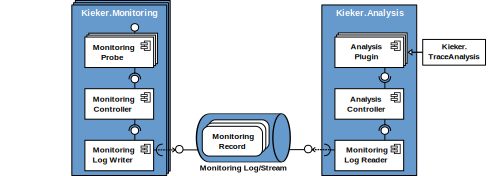
\includegraphics[width=0.81\textwidth]{images/kiekerComponentDiagram-woCloud-bw-w-record-newNames-withTraceAnalysis-colors}
			
			\caption{Overview of the framework components}
			\label{fig:KiekerComponentDiagram}
		\end{figure}
	
	\section{Download and Installation}
		
		The \Kieker{} download site\footnote{\KiekerDownloadURL{}} provides archives of the binary and source distribution, the Javadoc~API, as well as additional examples. The Java sources presented in this user guide, as well as pre-compiled binaries, are included in the \file{\exampleDir/} directory. The file \file{\mainJar{}} contains the \KiekerMonitoringPart{} and \KiekerAnalysisPart{} components, as well as the \KiekerTraceAnalysis{} tool. In addition to the \file{\mainJar{}} file, the \file{dist/} directory includes variants of this \file{.jar} files with integrated third-party libraries. Additional information on these \file{.jar} files and when to use them will follow later in this document.
		
	\section{Licensing}
		\Kieker{} is licensed under the Apache License, Version 2.0. You may obtain a copy of the license at \url{http://www.apache.org/licenses/LICENSE-2.0}. The \Kieker{} source and binary release archives include a number of third-party libraries. The \dir{lib/} directory of the release archives contains a \file{.LICENSE} file for each third-party library, pointing to the respective license text.	
		
	\section{Citing Kieker}\label{sec:ch1:citingKieker}
		When referencing Kieker resources in your publications, we would be happy if you respected the following guide lines:

		\begin{itemize}
			\item 
			When referencing the Kieker project, please cite our ICPE~2012~\cite{KiekerICPE2012} paper and/or our 2009 technical report~\cite{vanHoornRohrHasselbringWallerEhlersFreyKieselhorst2009TRContinuousMonitoringOfSoftwareServicesDesignAndApplicationOfTheKiekerFramework}. Also, you might want to add a reference to our web site (\url{http://kieker-monitoring.net/}) like~\cite{KiekerWebSite}. 
			\item 
			When referencing this user guide, e.g., when reprinting contents, please use a citation like~\cite{Kieker1.7UserGuide}.
		\end{itemize}

		\noindent At \url{http://kieker-monitoring.net/research/publications/} we provide entries for $\mathrm{B\scriptstyle IB}\!$\TeX{} and other bibliography systems.
		
	\section{Outline of this User Guide}
		The rest of this user guide is structured as followed. Chapter~\ref{chp:Quickstart-Example} contains a short quickstart example. In Chapter~\ref{chp:Kieker-Monitoring} we provide a detailed description of \KiekerMonitoringPart{} and its components, before presenting in Chapter~\ref{chp:Kieker-Analysis} the \KiekerAnalysisPart{} and its important parts. Various tools, which \Kieker{} already provides, can be found in Chapter~\ref{chp:Kieker-Tools}. The \hyperlink{hypertarget:appendix}{Appendix} finally includes additional resources, e.g., how to use the JMS writers and readers.
  \chapter{Kieker Monitoring}\label{chp:Kieker-Monitoring}
	\section{The Concept behind the Monitoring}
		\subsection{Data Flow}
		\subsection{Monitoring Components}
	\section{How to Monitor Applications}
		\subsection{Manual Probes}
		\subsection{Aspect Oriented Probes}
		\subsection{Monitoring within Java EE Applications}
			\subsubsection{Spring Probes}
			\subsubsection{Aspect Oriented Probes}
			\subsubsection{SOAP Interceptors}
		\subsection{Periodic Samplers}
			\subsubsection{Sigar}
	\section{Creating and Controlling the Monitoring}
		\subsection{Time Sources}
		\subsection{Adaptive Monitoring}
		\subsection{JMX MBean Access}
	\section{Development of own Monitoring Components}
		\subsection{Records}
		\subsection{Probes}
		\subsection{Writers}
  \chapter{Kieker Analysis}\label{chp:Kieker-Analysis}
	\section{The Concept behind the Analysis}
		\subsection{Data Flow}
		\subsection{Analysis Components}
	\section{Creating and Controlling the Analysis}
	\section{Development of own Analysis Components}
		\subsection{Readers}
		\subsection{Filters}
		\subsection{Repositories}
  \chapter{Kieker Tools}\label{chp:Kieker-Tools}
	\section{Trace Analysis}
		\subsection{Textual Trace and Equivalence Class Representations}
			\subsubsection{Execution Traces}
			\subsubsection{Message Traces}
			\subsubsection{Trace Equivalence Classes}
		\subsection{Sequence Diagrams}
			\subsubsection{Deployment-Level Sequence Diagrams}
			\subsubsection{Assembly-Level Sequence Diagram}
		\subsection{Call Trees}
			\subsubsection{Trace Call Trees}
			\subsubsection{Aggregated Call Trees}
		\subsection{Dependency Graphs}
			\subsubsection{Container Dependency Graphs}
			\subsubsection{Component Dependency Graphs}
			\subsubsection{Operation Dependency Graphs}
			\subsubsection{Response Times}
		\subsection{HTML Output of the System Model}	
			
	\section{Replay Monitoring Logs}
	\section{Convert Monitoring Timestamps}
	\section{KAX Viz}
	\section{KAX Runner}
	\section{TSLib \& OPAD}
	\newpage
	\section{Kieker WebGUI}\label{chp:Kieker-WebGUI}
		\subsection{Features}
		\subsection{Quickstart Example}
		\subsection{Detailed Introduction}
  \appendix
	\phantomsection
	\addcontentsline{toc}{chapter}{Appendix}\hypertarget{hypertarget:appendix}{}
	\addtocontents{toc}{\protect\setcounter{tocdepth}{-1}}

	\chapter{JMS}
		\section{OpenJMS}
		\section{ActiveMQ}
		\section{HornetQ}
		
	\chapter{Sigar}
  
  % suppress appendix chapters in toc:
  \addtocontents{toc}{\protect\setcounter{tocdepth}{0}}

\bibliographystyle{abbrvnatAvanhoorn} % alpha
\bibliography{bibliography}
\end{document}

